%==============================================================================
% locality-evaluation.tex
%==============================================================================

\chapter{Evaluation}
\label{chap:locality-evaluation}

We evaluate the performance of the different queue implementations
when used by the intervals scheduler with a variety of parallel Java
Grande Forum benchmarks (Appendix \ref{chap:appendix-benchmarks}) on
two different machines:

\begin{itemize}
\item Intel Core2 Duo with one processor and two cores, running Ubuntu
  10.04 64-bit with kernel 2.6.32 and Sun Hotspot JDK 1.6.0\_20
  (Appendix \ref{sec:experimental-setup-marvin})
\item Intel Nehalem with two processors and eight cores, running
  Ubuntu 9.04 64-bit with kernel 2.6.29 and Sun Hotspot JDK 1.6.0\_20
  (Appendix \ref{sec:experimental-setup-mafushi})
\end{itemize}

Both machines invoke the JVM with the following parameters:

\begin{lstlisting}
  -server -Xmx2048M -Xms2048M -Xss8m
\end{lstlisting}

The execution time reported is the average of the three best benchmark
iterations from ten separate invocations.

\begin{figure}[!ht]
  \centering
  \subfloat[Results for the Intel Core2 Duo machine]{
    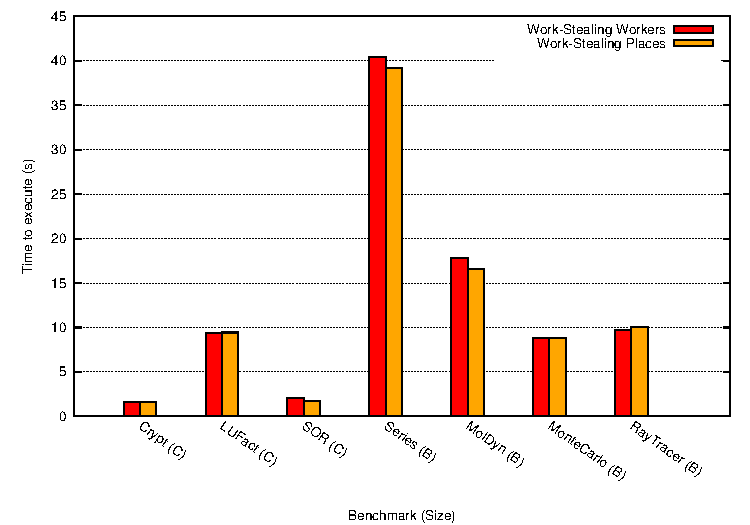
\includegraphics[width=0.5\linewidth]{locality-evaluation/marvin-jgf}
    \label{fig:locality-evaluation-marvin-jgf}
  }
  \subfloat[Results for the Intel Nehalem machine]{
    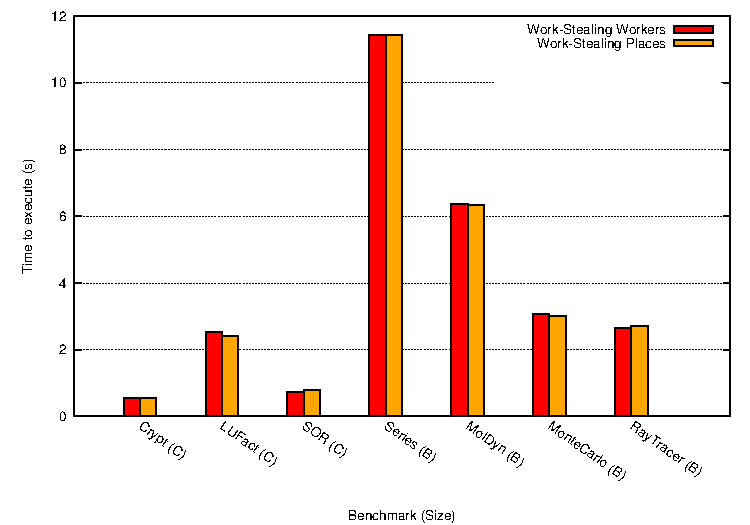
\includegraphics[width=0.5\linewidth]{locality-evaluation/mafushi-jgf}
    \label{fig:locality-evaluation-mafushi-jgf}
  }
  \caption[Work-Stealing Workers compared to Work-Stealing Places]{JGF
    benchmarks using \emph{Work-Stealing Workers} compared to
    \emph{Work-Stealing Places} running on our Intel Core2 Duo
    (Appendix \ref{sec:experimental-setup-marvin}) and Intel Nehalem
    (Appendix \ref{sec:experimental-setup-mafushi}) test machines}
  \label{fig:queues-performance-threads}
\end{figure}

\todo{Finish chapter ``Evaluation''}

\section{Locality-Aware Benchmarks}

We evaluate the locality-aware implementation of \emph{intervals} on a
variety of benchmarks. To reduce the impact of JVM overheads in the
evaluation, including JIT compilation and garbage collection, the
execution time reported is the average of the three best benchmark
iterations from three separate VM incocations. Each VM invocation
performs 10 benchmark iterations.

The JVM used on both machines described in appendix
\ref{chap:experimental-setup} is Sun Hotspot JDK 1.6. In both cases,
the JVM was invoked with the following parameters:

\begin{verbatim}
    -server -Xmx4096M -Xms4096M -Xss8m -XX:+UseNUMA
\end{verbatim}

The following benchmarks were first written to use threads and then
ported over to use \emph{intervals}.

\subsection*{Cache-Stress Test}

\todo{Describe benchmark ``Cache-Stress Test''}

\subsection*{Merge Sort}

\todo{Describe benchmark ``Merge Sort''}

\subsection*{Block Matrix Multiplication}

\todo{Describe benchmark ``Block Matrix Multiplication''}


%%% Local Variables: 
%%% mode: latex
%%% TeX-master: "thesis"
%%% End: 
